\documentclass{article}
\usepackage[paperwidth=10in,paperheight=5.625in,margin=0pt]{geometry}
\usepackage{tikz}
\usetikzlibrary{arrows.meta,positioning,fit,calc}
\pagestyle{empty}
\setlength{\parindent}{0pt}
\setlength{\topskip}{0pt}
\setlength{\parskip}{0pt}

\begin{document}
\thispagestyle{empty}%
\noindent\hspace*{0pt}%
\vbox to \paperheight{\vss\hbox to \paperwidth{\hss%
\resizebox{\paperwidth}{\paperheight}{%
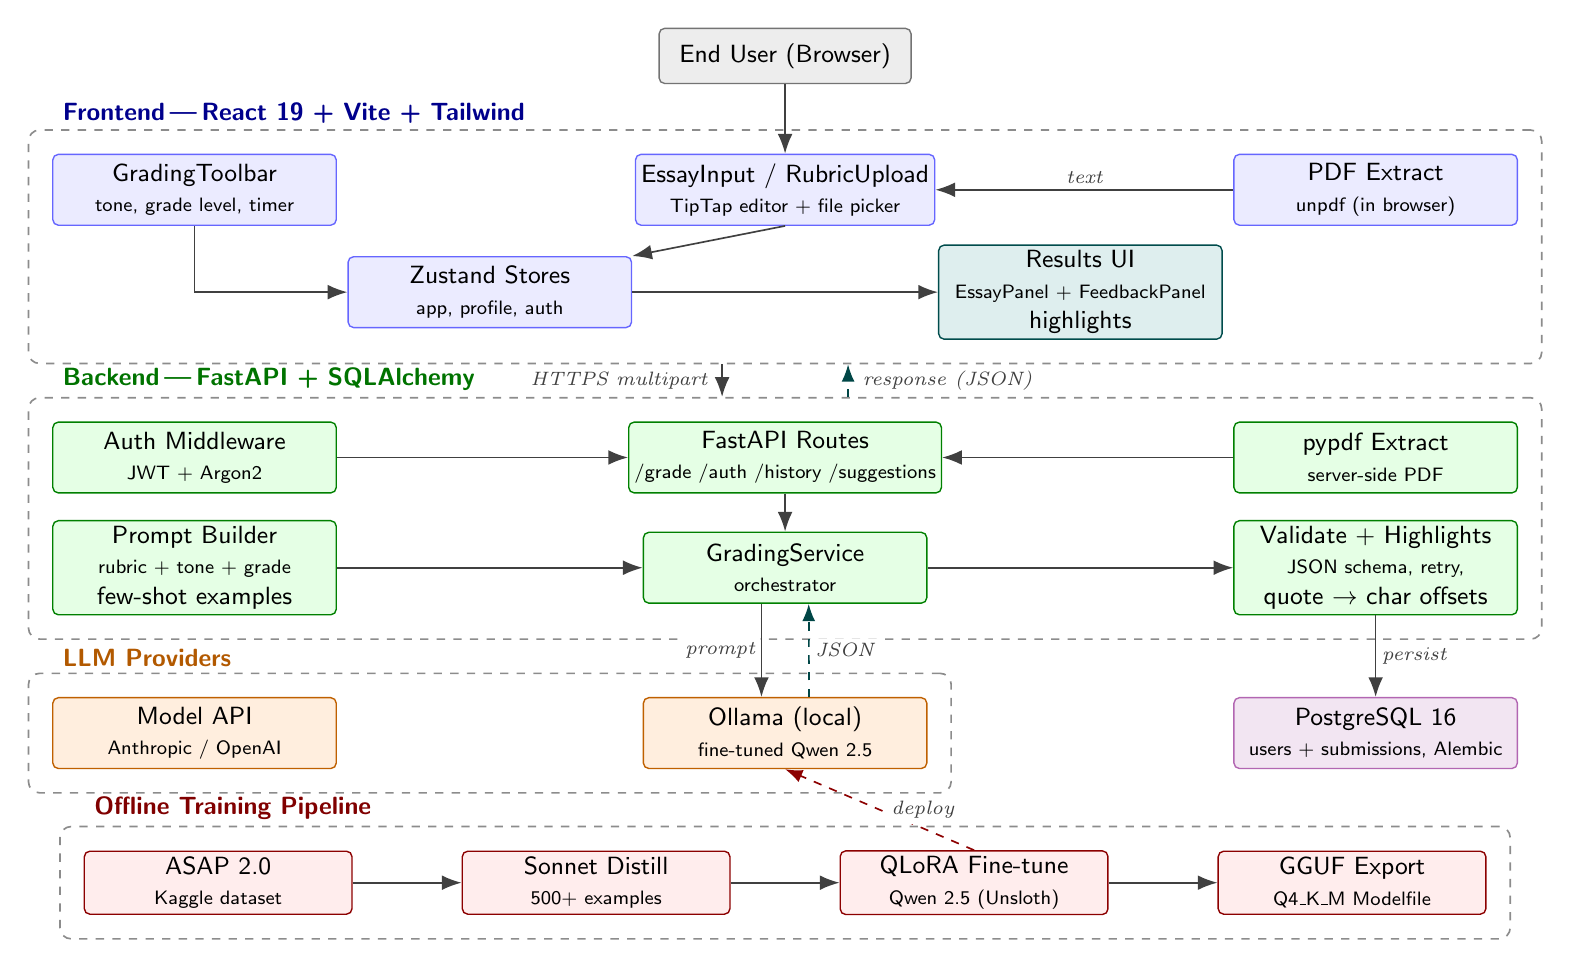
\begin{tikzpicture}[
  font=\sffamily\small,
  unit/.style={
    draw, rounded corners=2pt, align=center,
    minimum height=9mm, minimum width=36mm,
    fill=white, line width=0.5pt, inner sep=2pt
  },
  fe/.style    ={unit, fill=blue!8,    draw=blue!60},
  be/.style    ={unit, fill=green!10,  draw=green!50!black},
  llm/.style   ={unit, fill=orange!13, draw=orange!75!black},
  store/.style ={unit, fill=violet!10, draw=violet!60},
  result/.style={unit, fill=teal!13,   draw=teal!60!black},
  user/.style  ={unit, fill=black!7,   draw=black!55, minimum width=32mm, minimum height=7mm},
  train/.style ={unit, fill=red!7,     draw=red!55!black, minimum width=34mm, minimum height=8mm},
  group/.style ={draw, rounded corners=4pt, dashed, line width=0.6pt, draw=black!45, inner sep=3mm},
  flow/.style  ={-{Latex[length=2.5mm]}, semithick, draw=black!75},
  back/.style  ={-{Latex[length=2.2mm]}, semithick, dashed, draw=teal!55!black},
  deploy/.style={-{Latex[length=2.2mm]}, semithick, dashed, draw=red!55!black},
  lbl/.style   ={font=\scriptsize\itshape, inner sep=2pt, fill=white, text=black!75, align=center, rounded corners=1pt},
  glabel/.style={font=\sffamily\bfseries\small, inner xsep=4pt, inner ysep=0pt}
]

% =================== USER ===================
\node[user] (user) at (0, 5.7) {End User (Browser)};

% =================== FRONTEND ===================
\node[fe] (toolbar)   at (-7.5, 4.0) {GradingToolbar\\\scriptsize tone, grade level, timer};
\node[fe] (input)     at ( 0.0, 4.0) {EssayInput / RubricUpload\\\scriptsize TipTap editor + file picker};
\node[fe] (clientpdf) at ( 7.5, 4.0) {PDF Extract\\\scriptsize unpdf (in browser)};

\node[fe]     (stores)  at (-3.75, 2.7) {Zustand Stores\\\scriptsize app, profile, auth};
\node[result] (results) at ( 3.75, 2.7) {Results UI\\\scriptsize EssayPanel + FeedbackPanel\\highlights};

\node[group, fit=(toolbar)(input)(clientpdf)(stores)(results),
  label={[glabel, anchor=south west, text=blue!55!black, xshift=3mm, yshift=2pt]north west:Frontend\,—\,React 19 + Vite + Tailwind}] (feg) {};

% =================== BACKEND ===================
\node[be] (auth)   at (-7.5, 0.6) {Auth Middleware\\\scriptsize JWT + Argon2};
\node[be] (routes) at ( 0.0, 0.6) {FastAPI Routes\\\scriptsize /grade  /auth  /history  /suggestions};
\node[be] (pypdf)  at ( 7.5, 0.6) {pypdf Extract\\\scriptsize server-side PDF};

\node[be] (prompt)   at (-7.5, -0.8) {Prompt Builder\\\scriptsize rubric + tone + grade\\few-shot examples};
\node[be] (service)  at ( 0.0, -0.8) {GradingService\\\scriptsize orchestrator};
\node[be] (validate) at ( 7.5, -0.8) {Validate + Highlights\\\scriptsize JSON schema, retry,\\quote $\to$ char offsets};

\node[group, fit=(auth)(routes)(pypdf)(prompt)(service)(validate),
  label={[glabel, anchor=south west, text=green!45!black, xshift=3mm, yshift=2pt]north west:Backend\,—\,FastAPI + SQLAlchemy}] (beg) {};

% =================== EXTERNAL: LLM + DB ===================
\node[llm]   (api) at (-7.5, -2.9) {Model API\\\scriptsize Anthropic / OpenAI};
\node[llm]   (oll) at ( 0.0, -2.9) {Ollama (local)\\\scriptsize fine-tuned Qwen 2.5};
\node[store] (db)  at ( 7.5, -2.9) {PostgreSQL 16\\\scriptsize users + submissions, Alembic};

\node[group, fit=(api)(oll),
  label={[glabel, anchor=south west, text=orange!70!black, xshift=3mm, yshift=2pt]north west:LLM Providers}] (llmg) {};

% =================== TRAINING PIPELINE ===================
\node[train] (ds)   at (-7.2, -4.8) {ASAP 2.0\\\scriptsize Kaggle dataset};
\node[train] (dist) at (-2.4, -4.8) {Sonnet Distill\\\scriptsize 500+ examples};
\node[train] (lora) at ( 2.4, -4.8) {QLoRA Fine-tune\\\scriptsize Qwen 2.5 (Unsloth)};
\node[train] (gguf) at ( 7.2, -4.8) {GGUF Export\\\scriptsize Q4\_K\_M Modelfile};

\node[group, fit=(ds)(dist)(lora)(gguf),
  label={[glabel, anchor=south west, text=red!50!black, xshift=3mm, yshift=2pt]north west:Offline Training Pipeline}] (tg) {};

% =================== ARROWS ===================
% User -> EssayInput
\draw[flow] (user) -- (input);

% Frontend internal flow
\draw[flow] (clientpdf) -- node[lbl, above]{text} (input);
\draw[flow] (toolbar.south)   |- (stores.west);
\draw[flow] (input.south)     -- (stores.north east);
\draw[flow] (stores) -- (results);

% Frontend <-> Backend (parallel arrows between group boundaries)
\draw[flow] ([xshift=-8mm]feg.south) -- node[lbl, midway, anchor=east, xshift=-3pt]{HTTPS multipart} ([xshift=-8mm]beg.north);
\draw[back] ([xshift= 8mm]beg.north) -- node[lbl, midway, anchor=west, xshift= 3pt]{response (JSON)} ([xshift= 8mm]feg.south);

% Backend internal flow
\draw[flow] (auth.east)   -- (routes.west);
\draw[flow] (pypdf.west)  -- (routes.east);
\draw[flow] (routes)      -- (service);
\draw[flow] (prompt.east) -- (service.west);
\draw[flow] (service.east)-- (validate.west);

% Backend <-> LLM (parallel: prompt down, JSON back)
\draw[flow] ([xshift=-3mm]service.south) -- node[lbl, left, midway]{prompt} ([xshift=-3mm]oll.north);
\draw[back] ([xshift= 3mm]oll.north)     -- node[lbl, right, midway]{JSON}   ([xshift= 3mm]service.south);

% Backend -> Postgres
\draw[flow] (validate.south) -- node[lbl, right]{persist} (db.north);

% Training pipeline -> Ollama (deployment)
\draw[deploy] (lora.north) -- node[lbl, right=2pt]{deploy} (oll.south);

% Training pipeline internal flow
\draw[flow] (ds)   -- (dist);
\draw[flow] (dist) -- (lora);
\draw[flow] (lora) -- (gguf);

\end{tikzpicture}%
}%
\hss}\vss}%
\end{document}
